\documentclass[10pt,a4paper]{article}
\usepackage[T1]{fontenc}
\usepackage[utf8]{inputenc}
\usepackage{newtxtext,newtxmath}
\usepackage[a4paper,left=15mm,right=15mm,top=13mm,bottom=5mm]{geometry}
\usepackage{microtype,graphicx,multicol,tikz,caption,titlesec}
\usepackage[hidelinks]{hyperref}
\usepackage[backend=biber,style=numeric-comp,sorting=none,giveninits=true,
  maxbibnames=2,minbibnames=1,doi=false,url=false,isbn=false,eprint=false]{biblatex}
\addbibresource{references.bib}
\usetikzlibrary{arrows.meta,positioning,calc}
\definecolor{accent}{HTML}{204F46}
\definecolor{pale}{HTML}{F3F6F4}
\definecolor{rulegray}{HTML}{88968F}
\hypersetup{pdftitle={LabOpsBench: Benchmarking AI Agents for Laboratory Configuration and Experiment Scheduling},
  pdfauthor={Ryoma Yamamoto, Haruki Nakajima},
  pdfsubject={Hackathon extended abstract; feat/poc-integration at 00e8c4f}}
\pagestyle{empty}
\setlength{\parindent}{1em}
\setlength{\parskip}{0pt}
\setlength{\columnsep}{6mm}
\setlength{\multicolsep}{3.5pt}
\setlength{\emergencystretch}{1em}
\titleformat{\section}{\normalsize\bfseries}{\thesection}{0.55em}{}
\titlespacing*{\section}{0pt}{5pt}{2pt}
\captionsetup{font=small,labelfont=bf,labelsep=period,position=bottom,skip=-3pt,hypcap=false}
\setlength{\bibitemsep}{0.3pt}
\setlength{\bibparsep}{0pt}
\renewcommand*{\bibfont}{\fontsize{7}{8}\selectfont}
\DeclareFieldFormat{title}{\iffieldundef{doi}
  {\iffieldundef{url}{#1}{\href{\thefield{url}}{#1}}}
  {\href{https://doi.org/\thefield{doi}}{#1}}}
\DeclareFieldFormat[article]{title}{\iffieldundef{doi}
  {#1}{\href{https://doi.org/\thefield{doi}}{#1}}}
\renewbibmacro*{url+urldate}{}
\renewbibmacro*{in:}{}
\AtEveryBibitem{\clearfield{month}\clearfield{day}\clearfield{urlyear}\clearfield{urlmonth}\clearfield{urlday}\clearfield{issn}\clearfield{number}}

\begin{document}
\fontsize{10}{12}\selectfont
{\centering
  {\fontsize{16}{17.5}\selectfont\bfseries LabOpsBench: Benchmarking AI Agents for\\
  Laboratory Configuration and Experiment Scheduling\par}
  \vspace{2pt}
  {\normalsize Ryoma Yamamoto, Haruki Nakajima\par}
}
\vspace{3pt}

\begin{multicols}{2}
\section{Motivation: Why This Benchmark?}
Self-driving laboratories (SDLs) automate experiments and use the results to choose what to test next~\cite{tom2024}.
Language-model agents also execute robotic experiments, as demonstrated by Coscientist and ACRA (2026)~\cite{boiko2023,pagel2026}.
International efforts to build and scale SDL infrastructure include Canada's \href{https://acceleration.utoronto.ca/news/u-of-t-receives-200-million-grant-to-support-acceleration-consortiums-self-driving-labs-research}{\textcolor{accent}{Acceleration Consortium}} and autonomous-laboratory initiatives under the US \href{https://www.cmu.edu/news/stories/archives/2026/july/connecting-autonomous-laboratories-to-speed-scientific-advancement}{\textcolor{accent}{Genesis Mission}} and Japan's \href{https://www.jst.go.jp/program/arise/pdf/arise_siryo_st.pdf\#page=8}{\textcolor{accent}{ARiSE programme}}.

Cloud laboratories offer shared instruments remotely, without requiring laboratory ownership~\cite{arias2024}.
Scheduling at scale requires respecting workflow dependencies and instrument capacity~\cite{zhou2026} while coordinating shared transport and space.
These constraints motivate evaluating agents' equipment configuration and job prioritization.

\columnbreak
\section{Benchmark Environment and Policy Interface}
We developed LabOpsBench, a simulation-based benchmark that evaluates how AI agents select equipment configurations and prioritize predefined experimental jobs.
Jobs comprise dependent operations with fixed durations and required capabilities.
The simulator models instruments, robot arms, autonomous mobile robots (AMRs), queues, and finite buffers.
Its 14 scenarios span small cells to a facility with 32 instruments, 32 arms, and 64 jobs (Fig.~\ref{fig:loop}).

At each decision point, policies receive unfinished jobs, including future arrivals, and the laboratory state.
In this track, they return priorities and select configurations or equipment exchanges from shared candidates.
The engine validates decisions, dispatches feasible operations, and controls robot motion.
\end{multicols}

\par\vspace{3mm}
\noindent\begin{minipage}{\textwidth}
\centering
% All labels/arrows are vector graphics. Images are genuine recorded UI replays.
% Set \LabFigureFrame to 0 to compare the otherwise identical unframed variant.
\providecommand{\LabFigureFrame}{1}
\begin{tikzpicture}[x=1mm,y=1mm,>=Latex,
  every node/.style={inner sep=0,align=left,font=\fontsize{8.4}{9.5}\selectfont},
  flow/.style={-{Latex[length=3.1mm,width=2.8mm]},draw=accent,
    line width=2.2pt,line cap=round},
  outline/.style={draw=rulegray,line width=.55pt,rounded corners=2mm}]
\path[use as bounding box] (0,0) rectangle (180,82);
\ifnum\LabFigureFrame=1
  \draw[draw=rulegray!75,line width=.6pt,rounded corners=3mm,fill=pale!55] (.2,.2) rectangle (179.8,81.8);
\fi
\node[anchor=west,font=\fontsize{9}{10}\selectfont\bfseries,text=accent] at (5,77.5)
  {LABOPSBENCH: A SHARED EVALUATION LOOP};

% One shared engine; the inset contains two illustrative, independently run cases.
\draw[outline,fill=white] (5,18.5) rectangle (96,73);
\node[anchor=north west,font=\fontsize{10}{11}\selectfont\bfseries] at (8,70.5)
  {Laboratory Simulator (Engine)};
\node[anchor=north west,font=\fontsize{8.5}{9.5}\selectfont\bfseries,text=accent] at (8,65.2)
  {Example Scenarios (2 of 14)};
\path[fill=pale,rounded corners=1.5mm] (7.5,24) rectangle (93.5,61.2);
\node[anchor=north west,font=\fontsize{8.3}{9.2}\selectfont\bfseries] at (9,59.9)
  {(a) Two-Bay Cell};
\node[anchor=north west,font=\fontsize{8.3}{9.2}\selectfont\bfseries] at (48,59.9)
  {(b) 32-Station Hall};
\node[anchor=north west] at (9,56.3846)
  {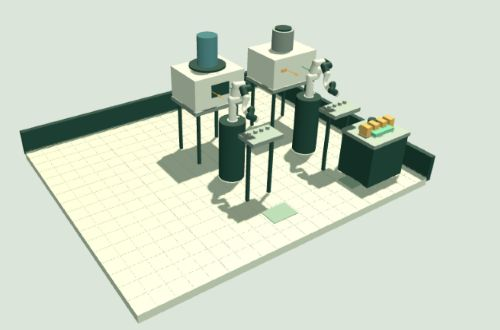
\includegraphics[width=35mm]{assets/lab-runtime-angle.jpg}};
% Exact viewport crop in TikZ: x=190..710, y=175..475 of a 1275x717 screenshot.
% No objects, colours or recorded geometry are added to the screenshot.
\begin{scope}[shift={(48,31)}]
  \clip (0,0) rectangle (44,25.3846);
  \node[anchor=north west] at (-16.076923,40.192307)
    {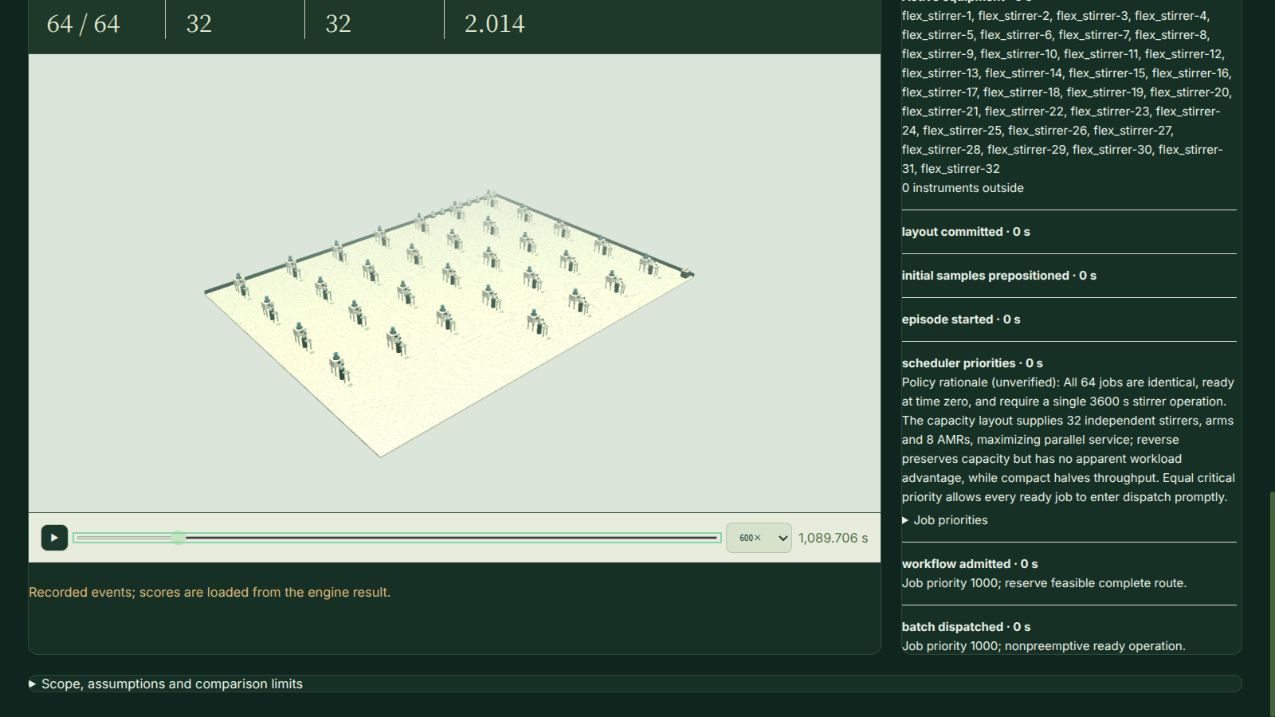
\includegraphics[width=107.884615mm]{assets/lab-runtime-large.png}};
\end{scope}
\node[anchor=north west,font=\fontsize{8}{9}\selectfont] at (9,30)
  {2 active instruments, 22 jobs\\$4\times3.4$ m; 34 stored outside};
\node[anchor=north west,font=\fontsize{8}{9}\selectfont] at (48,30)
  {32 instruments, 32 arms\\$32\times24$ m; 64 jobs, 8 AMRs};
\node[anchor=west,font=\fontsize{8.2}{9}\selectfont] at (8,21.5)
  {Validate $\rightarrow$ dispatch $\rightarrow$ advance simulated time};

% Observation -> policy -> action forms the right side of the loop.
\draw[outline,fill=white] (104,53) rectangle (175,73);
\node[anchor=north west,font=\fontsize{8.8}{9.8}\selectfont\bfseries] at (107,70.5)
  {INPUT: Observation at $t_k$};
\node[anchor=north west] at (107,65.5)
  {\textbf{Jobs:} arrivals, dependencies, durations\\
   \textbf{Lab:} layout, occupancy, resource limits\\
   \textbf{Menu:} public candidates; prior receipts};
\draw[fill=accent,draw=accent,rounded corners=2mm] (111,39.5) rectangle (168,48.5);
\node[text=white,anchor=center,align=center,font=\fontsize{10.4}{11}\selectfont\bfseries] at (139.5,45.2)
  {AI AGENT / ALGORITHM};
\node[text=white,anchor=center,font=\fontsize{8}{9}\selectfont] at (139.5,41.4)
  {Select equipment and prioritize jobs};
\draw[outline,fill=white] (104,20.5) rectangle (175,35);
\node[anchor=north west,font=\fontsize{8.8}{9.8}\selectfont\bfseries] at (107,32.8)
  {OUTPUT: Structured Decision};
\node[anchor=north west] at (107,28)
  {$t=0$: design candidate $+$ job priorities\\
   Later: priorities $+$ keep / allowed exchange};
\draw[flow] (96,63)--(104,63);
\draw[flow] (139.5,53)--(139.5,48.5);
\draw[flow] (139.5,39.5)--(139.5,35);
\draw[flow] (104,25)--(96,25);

% Timeline is part of the figure, below the loop and inside its outer frame.
\draw[rulegray!55,line width=.4pt] (5,16.3)--(175,16.3);
\node[anchor=north west,font=\fontsize{8.2}{9.2}\selectfont\bfseries] at (5,14.2)
  {Decision\\Timing};
\draw[->,rulegray,line width=.7pt] (30,12.7)--(174,12.7);
\foreach \x/\lab in {34/{$t=0$},74/{$1{,}800$ s},114/{$3{,}600$ s}}{
  \fill[accent] (\x,12.7) circle (.75);
  \node[anchor=north,align=center,font=\fontsize{8.2}{9}\selectfont] at (\x,10.9){\lab};
}
\node[anchor=center,fill=pale!55,inner sep=.8mm] at (137,12.7){$\cdots$};
\fill[accent] (159,12.7) circle (.75);
\node[anchor=north,align=center,font=\fontsize{8.2}{9}\selectfont] at (159,10.9){Completion};
\node[anchor=south west,font=\fontsize{8}{9}\selectfont] at (5,3)
  {Calls pause the clock; at most 32 submissions including $t=0$. Score: total completion time (makespan).};
\end{tikzpicture}

\captionof{figure}{\textbf{A shared evaluation loop.}
  LLM agents, heuristics, and algorithms share the observation--decision--execution interface.
  Panels (a) and (b) show recorded replays of cases 12 and 03, two examples from the 14-scenario suite. Each run evaluates one scenario.}
\label{fig:loop}
\end{minipage}
\par\vspace{4.7mm}

\begin{multicols}{2}
\section{Evaluation Protocol and Pilot Setup}
At $t=0$, the policy selects equipment/layout and priorities; subsequent decisions update priorities or request permitted exchanges (Fig.~\ref{fig:loop}).
After the 32-submission cap, the last valid policy continues.
Exchanges wait for admitted jobs to finish and incur handling, movement, reconnection, and calibration time.
\emph{Makespan} includes final unloading; incomplete runs receive no finite completion score.

The pilot contains 50 selected, completed trials: three methods on ten scenarios and five on four additional challenges.
Within each scenario, methods share workload, seed, resource limits, and candidate-generation rules.
We adapted eight scheduling templates from three public LeMat-Synth annotation records~\cite{lederbauer2026,lematannotations}; equipment mappings and missing timings are modeling assumptions.
Chemical outcomes and transfer to physical laboratories remain unvalidated.
\columnbreak
\section{Pilot Results and Conclusions}
We compared \texttt{gpt-6-luna} (medium reasoning) and \texttt{jev-1.14.0} with FIFO, a reference heuristic, and a workload-aware algorithm on shared candidates.

Scenario 12 (36 owned instruments, two active bays, 22 jobs) yielded makespans of 4.860\,h (Luna), 5.459\,h (Jev), 5.068\,h (algorithm), and 7.661\,h (FIFO/reference).
In scenario 14 (layout/transport, 48 jobs), Jev and the algorithm required 0.683\,h versus Luna's 0.724\,h.
These single-trial results illustrate task-dependent performance; they do not establish general model rankings.

LabOpsBench links structured policy decisions to simulated laboratory execution and completion time.
This executable benchmark enables controlled comparisons of equipment configuration and scheduling strategies under shared resource constraints.
\end{multicols}

\par\vspace{3pt}
\noindent{\fontsize{8.5}{9.2}\selectfont\bfseries References}\par
\vspace{-2pt}
\begin{multicols}{2}
\printbibliography[heading=none]
\end{multicols}
\end{document}
